\section{First-Mover Flow versus the institutional toolkit}\label{sec:toolkit}

A selection signal has value for a portfolio manager only when it adds something the standard toolkit lacks. I build 13 cross-sectional comparables (Appendix~\ref{app:defs}) with FMF-N's construction, so that any difference comes from the signal, and add three allocations. The comparables cover the price factors, the sell-side signals in common use and two multi-factor blends.

\para{League table:} Of the 14 cross-sectional books, FMF-N has the highest full-period Sharpe (1.13) and Calmar (0.78) ratios (Table~\ref{tab:league}, Figure~\ref{fig:league}). Next are classic revision breadth (0.92 and 0.58), itself one of FMF-N's components, and the momentum + revisions blend (0.87 and 0.49). Plain 12-1 momentum gets 0.50 and 0.23. Betting-against-beta, low dispersion and reversal lose money in this universe.

\para{Where the toolkit fails:} Figure~\ref{fig:episodes} and Table~\ref{tab:episodes} cover five named episodes.
\begin{itemize}
  \item \emph{COVID crash:} Market $-35.5\%$, betting-against-beta $-15.2\%$, reversal $-7.7\%$; FMF-N $+12.0\%$.
  \item \emph{Vaccine rotation (November 2020):} In this momentum crash FMF-N returned $-5.8\%$, against $-8.2\%$ for both 12-1 and residual momentum.
  \item \emph{Feb-Mar 2021 growth sell-off:} FMF-N's worst episode ($-7.1\%$) was milder than for 12-1 momentum ($-10.5\%$) and time-series momentum ($-12.1\%$).
\end{itemize}

\para{Spanning:} Regressed on the market and all 13 comparables, FMF-N's alpha falls to 1.8\% ($t = 1.46$, $R^2 = 0.92$; Table~\ref{tab:spanning}). This test is circular, since two comparables contain FMF-N's components. Against the market and the 11 comparables not built from its components the alpha is 6.1\% a year ($t = 2.51$) over 2017--2021 and 7.5\% ($t = 3.86$) in DEV.

\begin{table}[t]
\centering\footnotesize
\caption{FMF-N and institutional comparables, identical construction (net of 5\,bp)}\label{tab:league}
\begin{adjustbox}{max width=\textwidth}\begin{tabular}{lrrrrrrrrr}
\toprule
 & \multicolumn{3}{c}{Sharpe} & \multicolumn{3}{c}{Calmar} & MaxDD & Beta & Corr.\\
\cmidrule(lr){2-4}\cmidrule(lr){5-7}
 & DEV & Hold. & Full & DEV & Hold. & Full & Full (\%) & Full & FMF-N\\
\midrule
FMF-N (this paper) & 0.98 & 1.33 & 1.13 & 0.79 & 1.14 & 0.78 & $-14.1$ & $-0.02$ & 1.00\\
Revision breadth (classic) & 0.57 & 1.28 & 0.92 & 0.38 & 1.08 & 0.58 & $-15.5$ & $-0.02$ & 0.95\\
Momentum + revisions blend & 0.78 & 1.01 & 0.87 & 0.52 & 0.73 & 0.49 & $-18.5$ & $-0.01$ & 0.90\\
Multi-factor: mom + low vol + reversal & 0.88 & 0.80 & 0.81 & 0.71 & 0.52 & 0.42 & $-14.3$ & $-0.09$ & 0.44\\
Low volatility (60d) & 0.37 & 0.80 & 0.56 & 0.21 & 1.18 & 0.37 & $-13.6$ & $-0.10$ & 0.04\\
12-1 momentum (Jegadeesh-Titman) & 0.63 & 0.43 & 0.50 & 0.42 & 0.24 & 0.23 & $-21.8$ & $-0.02$ & 0.71\\
Target-price upside (consensus) & 0.47 & 0.29 & 0.38 & 0.37 & 0.24 & 0.24 & $-12.1$ & 0.04 & $-0.38$\\
52-week-high proximity & $-0.36$ & 1.06 & 0.37 & $-0.16$ & 0.75 & 0.17 & $-18.2$ & $-0.09$ & 0.73\\
Target-price momentum (63d) & $-0.36$ & 0.68 & 0.19 & $-0.15$ & 0.44 & 0.07 & $-20.4$ & $-0.08$ & 0.71\\
Residual momentum (Blitz et al.) & 0.42 & 0.00 & 0.17 & 0.24 & $-0.04$ & 0.05 & $-24.1$ & $-0.06$ & 0.64\\
6-1 momentum & $-0.51$ & 0.55 & 0.06 & $-0.16$ & 0.32 & 0.00 & $-24.8$ & $-0.04$ & 0.67\\
Betting-against-beta (low beta) & $-0.28$ & 0.00 & $-0.15$ & $-0.17$ & $-0.05$ & $-0.07$ & $-32.2$ & 0.01 & 0.10\\
Short-term reversal (1m) & 0.25 & $-0.69$ & $-0.24$ & 0.16 & $-0.33$ & $-0.09$ & $-18.7$ & 0.04 & $-0.51$\\
Low analyst dispersion & $-0.36$ & $-0.74$ & $-0.53$ & $-0.19$ & $-0.50$ & $-0.20$ & $-27.7$ & $-0.13$ & $-0.15$\\
\midrule
\multicolumn{10}{l}{\emph{Allocation benchmarks}}\\
Equal-weight long-only (market) & 1.59 & 1.08 & 1.28 & 1.31 & 0.89 & 0.87 & $-38.1$ & 1.00 & $-0.02$\\
Inverse-vol long-only (naive risk parity) & 1.67 & 1.17 & 1.35 & 1.37 & 0.99 & 0.92 & $-37.2$ & 0.96 & $-0.01$\\
Time-series momentum 12-1 (CTA-style) & 0.89 & 0.86 & 0.86 & 0.57 & 0.89 & 0.54 & $-30.2$ & 0.61 & 0.29\\
RTB: original regime-timed breadth (gross) & 1.56 & 1.45 & 1.48 & 1.77 & 1.65 & 1.39 & $-13.6$ & 0.11 & 0.63\\
FMF-B20: FMF + explicit 0.2 beta budget & 1.56 & 1.73 & 1.62 & 1.82 & 2.17 & 1.66 & $-10.8$ & 0.17 & 0.89\\
\bottomrule
\end{tabular}\end{adjustbox}
\par\smallskip\begin{minipage}{0.97\textwidth}\footnotesize Cross-sectional comparables: top/bottom four, inverse-GJR weights, 42-session tranches, $\tau=0$, net of 5\,bp. Allocation benchmarks in their natural form. RTB gross; FMF-B20 adds a constant 0.2 beta budget to FMF-N.\end{minipage}
\end{table}

\begin{table}[t]
\centering\footnotesize
\caption{Named episodes: cumulative returns (\%)}\label{tab:episodes}
\begin{adjustbox}{max width=\textwidth}\begin{tabular}{lrrrrr}
\toprule
 & Q4-2018 & COVID crash & COVID rebound & Vaccine rotation & Growth sell-off\\
 & 10/03--12/24/18 & 02/19--03/23/20 & 03/24--06/08/20 & 11/06--11/30/20 & 02/12--03/08/21\\
\midrule
FMF-N & $-0.8$ & 12.0 & $-4.0$ & $-5.8$ & $-7.1$\\
12-1 momentum (Jegadeesh-Titman) & $-0.6$ & 12.2 & $-9.8$ & $-8.2$ & $-10.5$\\
Residual momentum (Blitz et al.) & 5.3 & 8.3 & $-11.1$ & $-8.2$ & $-10.4$\\
Low volatility (60d) & 2.6 & $-0.6$ & 2.8 & 2.8 & 1.2\\
Betting-against-beta (low beta) & 1.3 & $-15.2$ & 3.0 & $-1.0$ & $-1.7$\\
Short-term reversal (1m) & 1.9 & $-7.7$ & 2.4 & 4.0 & 1.1\\
Target-price upside (consensus) & 3.1 & $-3.7$ & 6.3 & 7.3 & 1.7\\
Revision breadth (classic) & $-1.7$ & 10.2 & $-2.3$ & $-7.4$ & $-6.1$\\
Multi-factor: mom + low vol + reversal & 4.2 & 6.0 & $-5.8$ & $-0.7$ & $-4.7$\\
Time-series momentum 12-1 (CTA-style) & $-23.3$ & $-18.9$ & 18.5 & $-3.5$ & $-12.1$\\
Equal-weight long-only (market) & $-24.8$ & $-35.5$ & 60.9 & 6.9 & $-9.4$\\
RTB: original regime-timed breadth & $-4.1$ & 11.9 & $-1.1$ & $-5.5$ & $-9.2$\\
\bottomrule
\end{tabular}\end{adjustbox}
\end{table}

\begin{figure}[t]
\centering
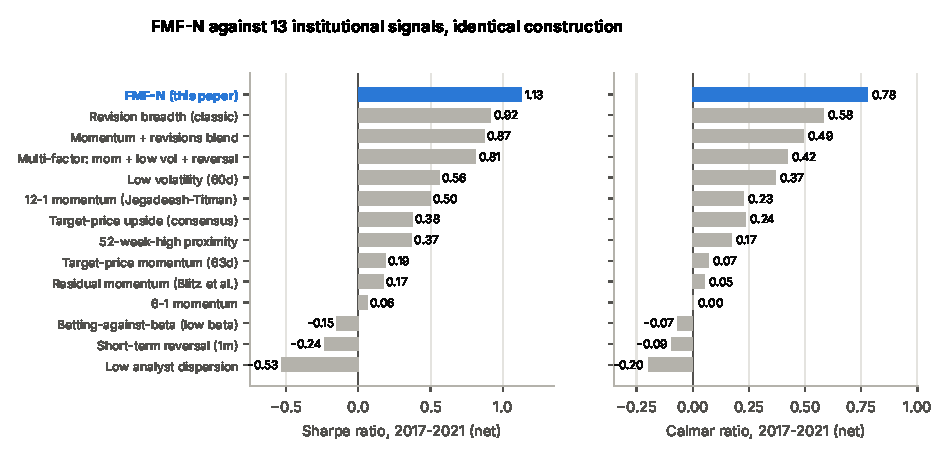
\includegraphics[width=\figw]{fig/fig08.pdf}
\caption{Full-period Sharpe and Calmar ratios of FMF-N and 13 institutional signals built through the identical construction.}\label{fig:league}
\end{figure}

\begin{figure}[t]
\centering
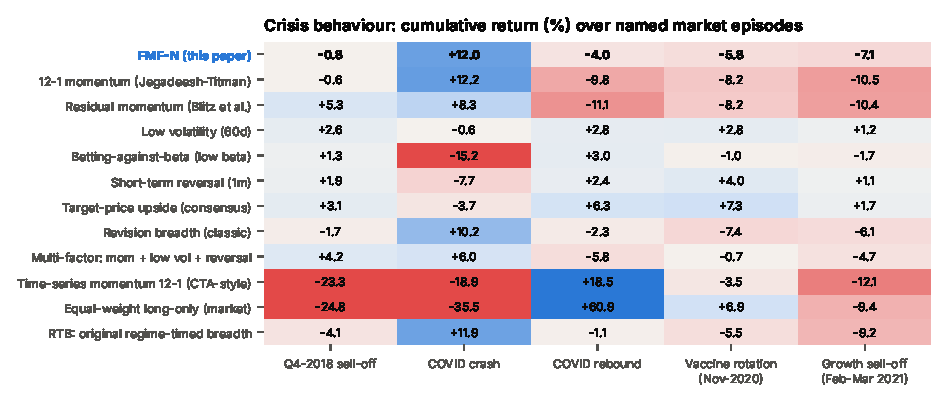
\includegraphics[width=\figw]{fig/fig09.pdf}
\caption{Cumulative return over named market episodes (blue: gain, red: loss).}\label{fig:episodes}
\end{figure}

\para{Blending:} Blended 50/50 with FMF-N, 16 of 18 comparables get a higher Sharpe ratio and 16 of 18 a higher Calmar ratio (Figure~\ref{fig:blend}). The two that do not are the books which already hold market beta (RTB and FMF-B20); their Calmar ratios come from the bull market

\para{Tranches and native form:} Slow tranches suit slow analyst-flow signals (classic breadth: full-period Sharpe 0.92 in tranches, 0.52 in native monthly form) but not every price signal (12-1 momentum: 0.74 native, 0.50 in tranches)

\begin{table}[t]
\centering\small
\caption{Spanning regressions of the weekly FMF-N return}\label{tab:spanning}
\begin{adjustbox}{max width=\textwidth}\begin{tabular}{llrrr}
\toprule
Regressors & Window & $\alpha$ (\% p.a.) & $t(\alpha)$ & $R^2$\\
\midrule
Market + all 13 comparables & DEV & 2.4 & 2.19 & 0.95\\
 & Holdout & 1.2 & 0.50 & 0.93\\
 & Full & 1.8 & 1.46 & 0.92\\
Market + 11 comparables not built from FMF components & DEV & 7.5 & 3.86 & 0.77\\
 & Holdout & 6.4 & 1.02 & 0.69\\
 & Full & 6.1 & 2.51 & 0.69\\
\bottomrule
\end{tabular}\end{adjustbox}
\par\smallskip\begin{minipage}{0.9\textwidth}\footnotesize OLS on non-overlapping weekly returns, HAC(4) errors. The first panel includes classic breadth and the momentum + revisions blend, both built from FMF-N's components.\end{minipage}
\end{table}

\begin{figure}[t]
\centering
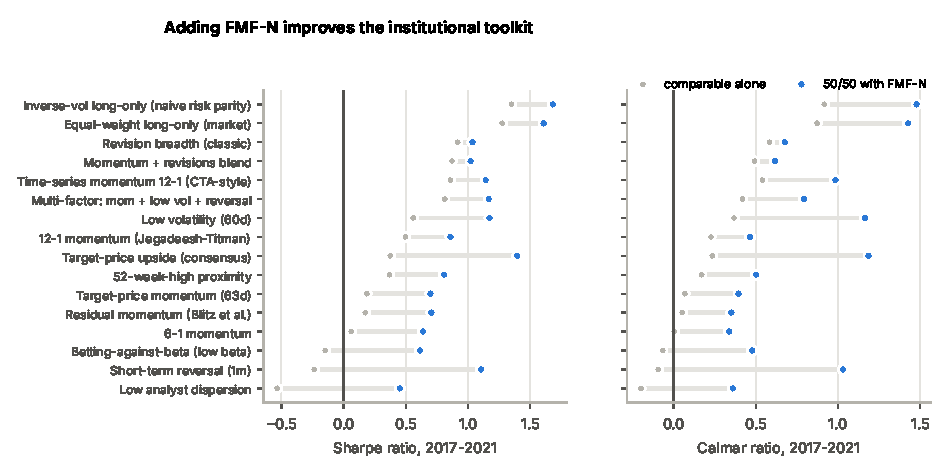
\includegraphics[width=\figw]{fig/fig10.pdf}
\caption{Full-period Sharpe and Calmar ratios of each comparable alone (grey) and blended 50/50 with FMF-N (blue).}\label{fig:blend}
\end{figure}
